\section{综合讨论与研究展望}
\subsection{由流程自动化转向研究有效性}
前述研究表明，知识增强、长期记忆与多代理协作分别处理不同瓶颈，系统能力来自其配合，而不是某个机制名称。
更强检索可以改善问题所依据的材料，长期记忆可以减少反复重建上下文，协作则可以组织专业工具与检查过程。
这些进展确实扩大了自动科研的任务范围。
然而，跨阶段组合也使局部错误更容易影响后续选择，因此评价对象应从单步回答继续扩展到研究依赖关系。

本文认为，科研系统值得长期保留的基本对象，应是具有明确依据和适用范围的研究判断。
每项关键判断关联其来源、实验条件和反证，后续任务才能知道哪些内容可以继续采用、哪些仍需验证。
当数据处理被修正时，系统应识别受影响的结果与结论，而不是只重新生成一篇措辞一致的报告。
这一要求将知识图谱的关联能力、记忆的版本维护和协作的返工控制联系起来，也为长期科研评价提供了更具体的观察对象。

\subsection{知识组织与研究记忆的互补关系}
课堂中关于图式知识组织和自主记忆的讨论，反映了两种不同需求。
图结构适合相对稳定的概念关联和跨文献主题，任务记忆则需要快速容纳尚不确定的尝试、解释与异常。
若全部内容都按稳定知识处理，新假设可能过早固化；若只保留自由对话，重要关系又难以持续利用。
因此，二者结合的关键不是采用相同存储格式，而是明确什么信息在何种条件下可以转入较稳定的知识状态。

一个可行方向是保留观察、解释和结论之间的依赖，让反证能够改变状态而不抹去历史。
常规记录可以压缩，影响研究方向的判断则保留更完整依据。
图\ref{fig:cycle}给出了本文的综合理解：检索和候选生成扩展探索范围，区分性实验提供新观察，
记忆更新再影响下一轮选择。
这一路径同时强调信息获取与认识修订，能够避免把已有判断在知识库和代理之间反复传递当成新的支持。

\begin{figure*}[t]\centering
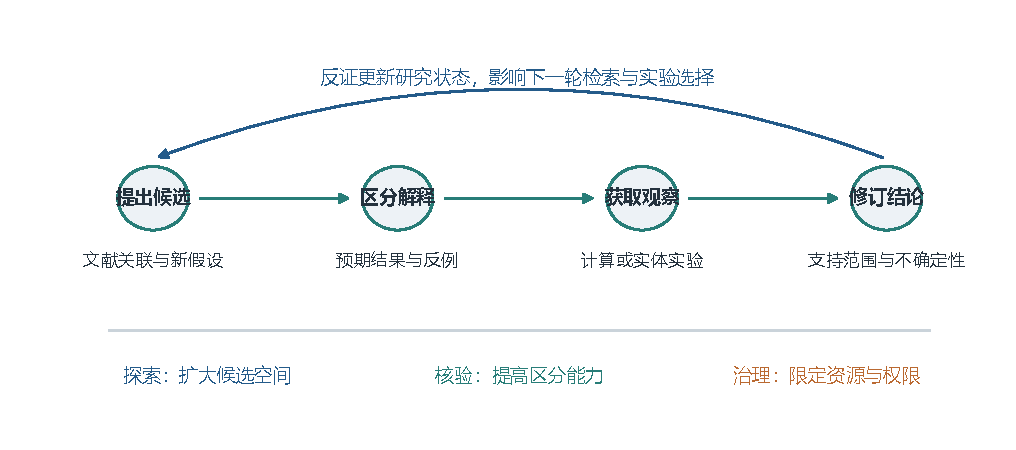
\includegraphics[width=\textwidth]{figures/review-evidence-cycle.pdf}
\caption{基于综述形成的研究闭环理解。候选生成、区分解释、外部观察与结论修订相互联系，
探索、核验和资源治理分别提供不同约束。该图为本文讨论框架，未声称已经实现或经新实验验证。}
\label{fig:cycle}\end{figure*}

\subsection{探索效率与验证成本的共同约束}
候选生成速度提高之后，系统瓶颈可能从提出想法转移到判断哪些想法值得继续研究。
更多代理能够产生更多方案，却未必增加实验资源或领域审查能力。
因此，研究预算需要同时覆盖探索与核验，并考虑不同候选能否被现有数据或低成本实验有效区分。
对于验证代价较高的问题，单纯增加候选数可能增加筛选负担，而不是提高科研效率。

验证也不应被简化为与已有共识的一致程度。
新假设往往超出现有结论，审查的作用是确认事实基础、逻辑关系与可检验条件，而非要求所有推测都已被证明。
允许系统明确保留“尚待检验”的判断，能够在探索空间与科学审慎之间形成更合理的平衡。
相应地，评价应分别报告新颖性、可行性和证据支持度，不宜由一个语言偏好分数替代。

\subsection{协作规模与人工参与的任务适配}
科研多代理更适合任务依赖复杂、工具异质且交付可检查的场景。
对于局部事实检索，增加角色可能主要增加通信成本；对跨学科设计，不同功能主体与专用工具之间的配合则更有价值。
因此，协作规模宜由任务结构和实际消融决定。
未来系统可以根据当前不确定性调整参与角色，而非从开始到结束维持固定人数和相同讨论模式。

人的作用也需要从简单的“是否介入”进一步细化。
问题选择、对照设计、异常解释和结论范围通常具有较高判断价值；常规检索、运行和材料整理则更适合交由工具处理。
在前者设置清晰检查点，有助于把有限专家时间用于最影响研究有效性的环节。
同时，评价需要记录人工输入与修改程度，才能判断系统是在替代劳动、放大已有能力，还是把工作转移到了未被计量的审查过程。

\begin{table*}[t]\centering\tabletext
\caption{由本文分析形成的可检验研究议题。以下为研究设计建议，未报告本项目新实验。}
\label{tab:agenda}
\begin{tabularx}{\textwidth}{@{}>{\raggedright\arraybackslash}p{32mm}YY@{}}\toprule
研究议题 & 可采用的对照设计 & 需要观察的结果\\\midrule
来源与状态管理的贡献 & 相同工具和预算下，比较无类型记忆与来源、状态可区分的记忆 & 错误重复、反证利用、关键判断可重建程度\\
协作结构的必要性 & 保留调用预算和权限，比较单代理、固定分工及动态调度 & 完成质量、通信开销、中断与返工分布\\
独立检查的有效性 & 保留角色数，改变检查者能访问的原文、数据与执行记录 & 缺陷识别、误报、修正成功和检查成本\\
人机协作的价值位置 & 记录并比较目标、实验设计及结果解释阶段的人工介入 & 质量改善、专家时间、修改量及研究者负担\\\bottomrule
\end{tabularx}\end{table*}

\subsection{长期评价与本文局限}
真实科研往往没有立即可知的唯一答案，目标也可能随新证据改变。
短任务基准适合比较局部能力，但对长期研究中的错误恢复、方向调整和失败价值覆盖不足。
未来评价应保留跨阶段轨迹，并在可行时加入独立执行者、预先保留任务及后续复查，
考察系统能否在新证据下更新既有结论，而不只是完成一次既定流程。

本文以知识、记忆和协作为主要分析线索，没有完整覆盖训练式多代理优化、基础模型训练和所有学科应用。
所引系统的模型、任务、工具与人工参与不同，本文不进行跨论文效应合并。
重绘数据图仅呈现原论文内部比较，转载谱图保留原始实验属性，均未作为本项目新结果。
此外，早期模型上的数值表现不代表当前系统水平；其揭示的评价问题需要在新模型和新任务中继续检验。

\section{结语}
大语言模型驱动的科研多智能体系统，正在将知识获取、工具执行和研究交流整合到持续工作流中。
检索增强改善外部知识的访问，层次与图组织支持跨材料综合，反思和分层记忆延续任务经历，
协作协议与搜索调度则组织多个主体在研究过程中的配合。
代表系统展示了从文献综合到计算实验、再到实体测量的多种路径，也说明不同科研活动需要不同形式的反馈与验证。

综合现有证据，协作规模、自动化覆盖和科研可信度应分别描述。
可靠系统需要保留来源、实验条件、失败尝试及修订依据。
知识与研究状态的协同维护、探索和验证资源的联合分配，以及关键节点的人机协作，
是值得持续研究的方向。
科研智能体的价值，最终应体现为更有效、更可复查的研究过程与产出。
